\section{Experiments}
\label{chap2-sec:experiments}

% Based on the theoretical results in Sections~\ref{chap2-sub:algorithms_theoretical_analysis} and \ref{chap2-sub:clip_theoretical_analysis}, we would like to pose the following questions:
To evaluate each component of our algorithms in Sections~\ref{chap2-sec:algorithms} and \ref{chap2-sec:double_clip} as well as our entire algorithms (i.e., \AlgOne, \AlgTwo, \AlgThree with double clipping), we pose the following three research questions:
%\begin{enumerate}
\begin{description}[leftmargin=9.75mm]
% \begin{itemize}[leftmargin=9.7mm]
    \item[RQ1.] 
    %\item 
    How do our three triangle counting algorithms 
    (i.e., \AlgOne, \AlgTwo, \AlgThree) in Section~\ref{chap2-sec:algorithms} compare with each other in terms of accuracy?
    \item[RQ2.] 
    %\item 
    How much does our double clipping technique in Section~\ref{chap2-sec:double_clip} decrease the estimation error?
    %increases the utility?
    \item[RQ3.] 
    %\item 
    How much do our entire algorithms reduce the communication cost, compared to the existing algorithm~\cite{Imola_USENIX21}, while keeping high utility (e.g., relative error $\ll 1$)?
% \end{enumerate}
\end{description}
% \end{itemize}
% To answer to the questions, we designed our experiments.
% We explain our experimental setup in Section~\ref{chap2-sub:setup}. 
% Note that we compare our entire algorithms with the two-rounds algorithm~\cite{Imola_USENIX21} 
% because one-round algorithms result in a very large estimation error, as shown in Appendix~\ref{chap2-sec:one-round}. 
% See Appendix~\ref{chap2-sec:one-round} for the comparison with one-round algorithms.
In Appendix~\ref{chap2-sec:one-round}, we also compare our entire algorithms with one-round algorithms.


% focus on the two-rounds algorithms in our experiments. 
% Below we explain our experimental set-up (Section~\ref{chap2-sub:setup}) and report results (Section~\ref{chap2-sub:results}) to answer to the three questions.

\subsection{Experimental Set-up}
\label{chap2-sub:setup}
In our experiments, we used two real graph datasets:

\smallskip
\noindent{\textbf{Gplus.}}~~The Google+ dataset~\cite{McAuley_NIPS12} (denoted by \GPlus{}) 
% includes a social graph collected from users who had shared circles. 
was collected from users who had shared circles. 
% includes publicly available network information collected from users who had shared circles. 
% ego-networks that represent Google+ users who had shared circles and whose network information is publicly available. 
From the dataset, we 
% extracted 
constructed 
a social graph $G=(V,E)$ with $107614$ nodes (users) and $12238285$ edges, where 
% an edge represents that a user follows or is followed by another one. 
edge $(v_i,v_j) \in E$ represents that $v_i$ follows or is followed by $v_j$. 
The average (resp.~maximum) degree in $G$ is $113.7$ (resp.~$20127$). 

\smallskip
\noindent{\textbf{IMDB.}}~~The IMDB (Internet Movie Database)~\cite{IMDB_GD05} (denoted by \IMDB{}) includes a bipartite graph between $896308$ actors and $428440$ movies. 
From this, we constructed a graph $G=(V,E)$ with $896308$ nodes (actors) and $57064358$ edges, where edge $(v_i,v_j) \in E$ represents that $v_i$ and $v_j$ have played in the same movie. 
The average (resp.~maximum) degree in $G$ is $63.7$ (resp.~$15451$). 
Thus, \IMDB{} is more sparse than \GPlus{}. 

\smallskip
In \conference{the full version \cite{Imola_arXiv22}}\arxiv{Appendix~\ref{chap2-sec:BAmodel}}, we also evaluate our algorithms using a synthetic graph based on the Barab\'{a}si-Albert model~\cite{NetworkScience}, which has a power-law degree distribution. 
%We report the results in 
%\conference{the full version \cite{Imola_arXiv22}}\arxiv{Appendix~\ref{chap2-sec:BAmodel}}.

% In our three triangle counting algorithms, we set 
% the ARR parameter $\mu$ so that $\mu$ in \AlgOne{} is equal to $\mu^2$ in \AlgTwo{} and also equal to $\mu^3$ in \AlgThree{}; i.e., $\CostDL{}$ is the same between the three algorithms. 
% Let $\mu^* = \mu$, $\mu^2$, and $\mu^3$ in \AlgOne{}, \AlgTwo{}, and \AlgThree{}, respectively. 
We evaluated our algorithms while changing $\mu^*$, where $\mu^* = \mu$, $\mu^2$, and $\mu^3$ in \AlgOne{}, \AlgTwo{}, and \AlgThree{}, respectively. 
$\CostDL{}$ is the same between the three algorithms. 
We typically 
set the total privacy budget $\epsilon$ to $\epsilon=1$ 
% or $2$ 
(at most $2$) 
because it is acceptable in many practical scenarios \cite{DP_Li}. 

In our double clipping, we set $\alpha = 150$ and $\beta = 10^{-6}$ so that both edge removal and triangle removal occur with a very small probability ($\leq 10^{-6}$ when $\epsilon_0 = 0.1$). 
% \commentT{Will write how to set $\td_i$ and $\kappa_i$ in double clipping.}
Then for each algorithm, we evaluated the relative error between the true triangle count $f_\triangle(G)$ and its estimate $\hf_\triangle(G)$. 
% (as described in Section~\ref{chap2-sub:LDP}). 
Since the estimate $\hf_\triangle(G)$ varies depending on the randomness of LDP mechanisms, we ran each algorithm $\tau \in \nats$ times ($\tau=20$ and $10$ for \GPlus{} and \IMDB{}, respectively) and averaged the relative error over the $\tau$ cases.

\subsection{Experimental Results}
\label{chap2-sub:results}

\smallskip
% \noindent{\textbf{Three Algorithms w/ Lap.}}~~
\noindent{\textbf{Performance Comparison.}}~~First, 
we 
% evaluated our algorithms with the Laplacian noise at the second round. 
evaluated our algorithms with the Laplacian noise. 
% and compared them with the existing two-rounds algorithm in \cite{Imola_USENIX21}. 
Specifically, we evaluated all possible combinations of our three algorithms with and without our double clipping (six combinations in total) and compared them with 
the existing two-rounds algorithm in~\cite{Imola_USENIX21}.  
% the algorithm in~\cite{Imola_USENIX21}.  
For algorithms with double clipping, we divided the total privacy budget $\epsilon$ as: 
% used $\frac{\epsilon}{10}$ for the adaptive edge clipping, and the remaining budget 
% $\epsilon_0: \epsilon_1: \epsilon_2 = 0.1: 0.45: 0.45$.
$\epsilon_0 = \frac{\epsilon}{10}$ and 
$\epsilon_1 = \epsilon_2 = \frac{9\epsilon}{20}$. 
Here, we set a very small budget ($\epsilon_0 = \frac{\epsilon}{10}$) for edge clipping because the degree has a small sensitivity (sensitivity$=1$). 
For algorithms without double clipping, we divided $\epsilon$ as $\epsilon_1 = \epsilon_2 = \frac{\epsilon}{2}$ and 
used the maximum degree $d_{max}$ as the global sensitivity. 
% We emphasize again that our algorithms with double clipping do not assume that $d_{max}$ is public.

\begin{figure}[t]
  \centering
  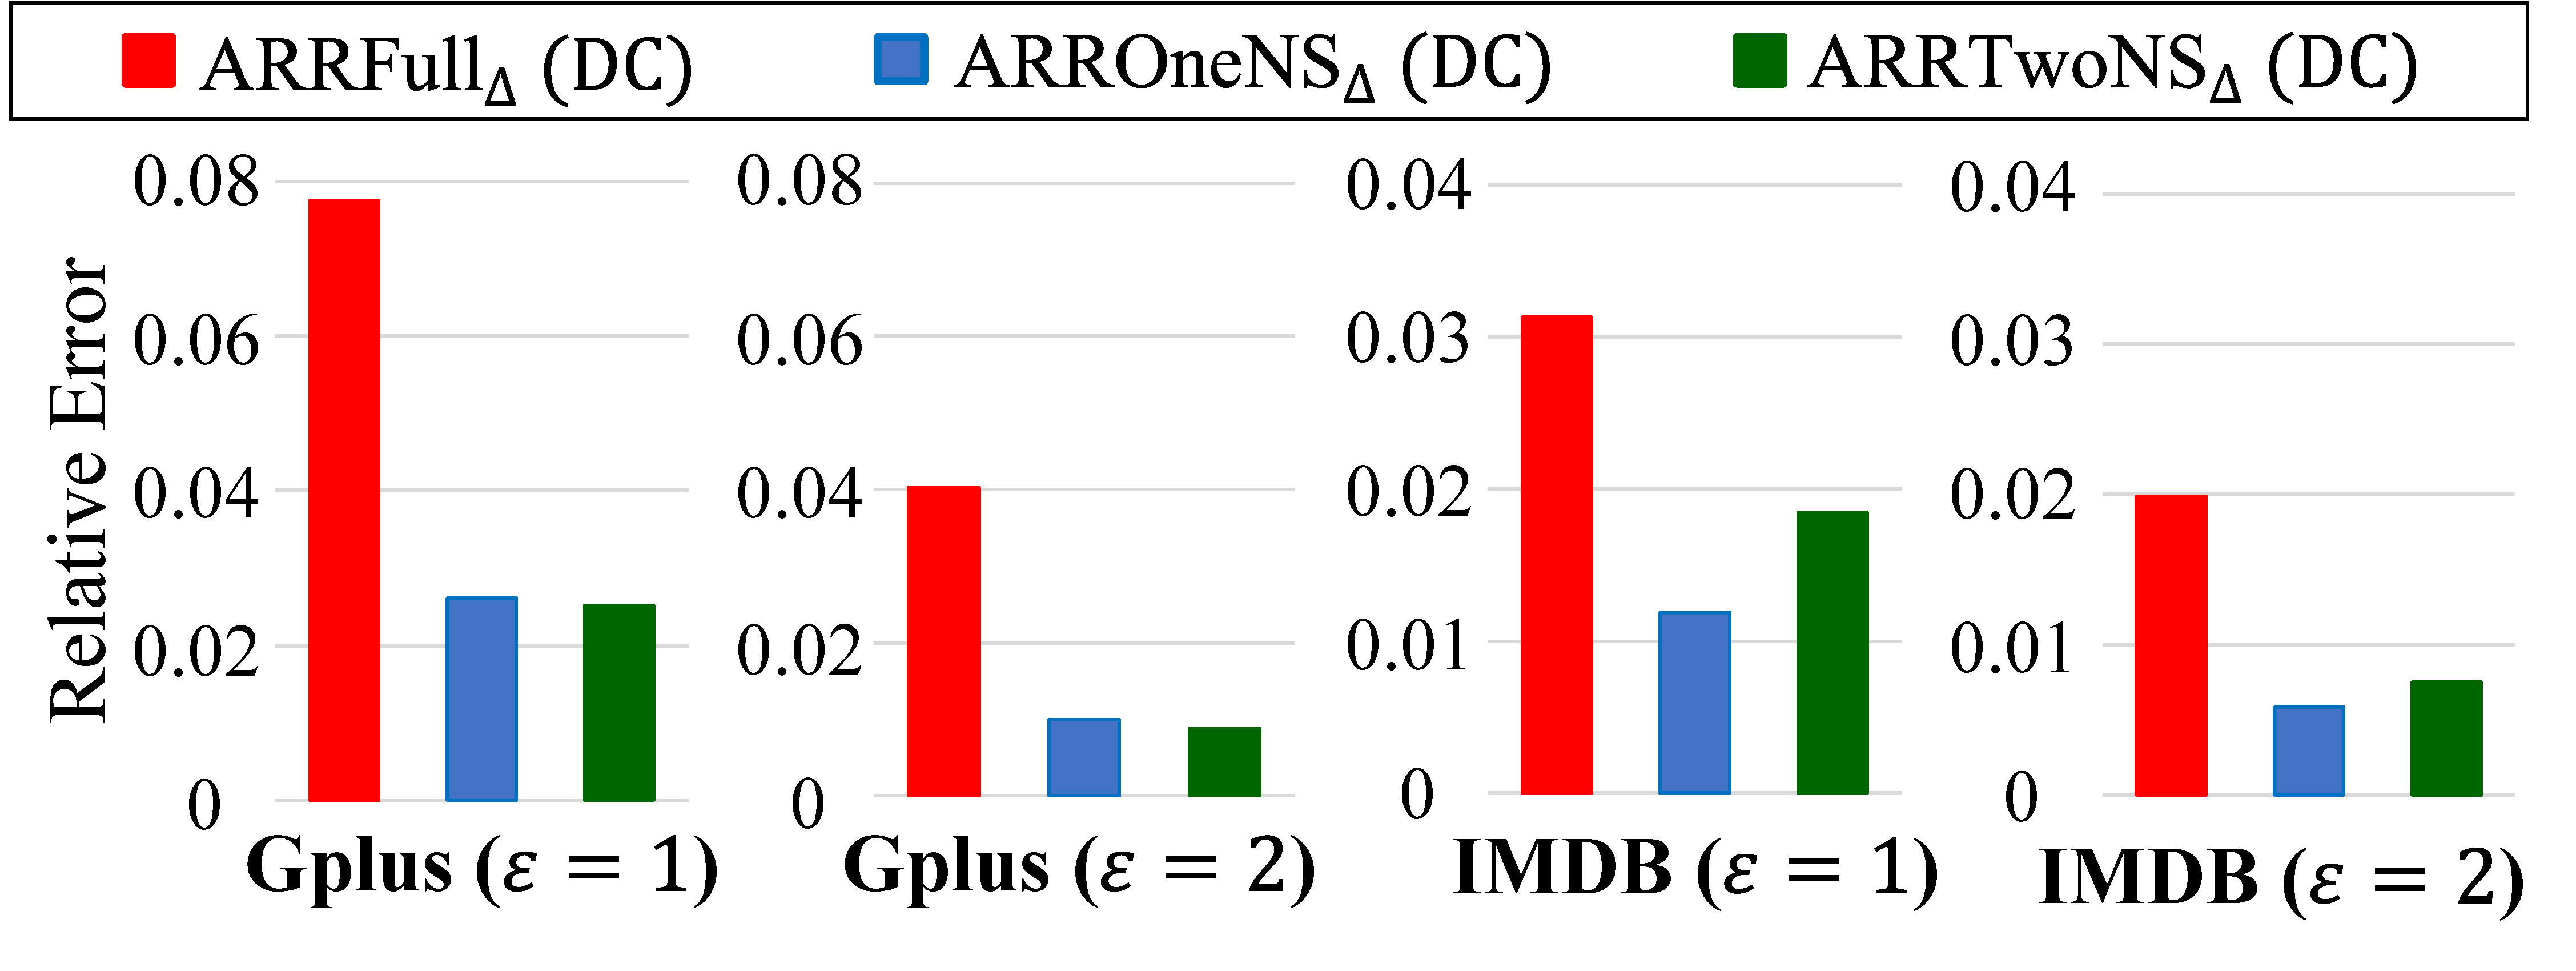
\includegraphics[width=0.96\linewidth]{fig/res2_w_Lap_abst2.pdf}
  \vspace{-6mm}
  \caption{Relative error of our three algorithms with double clipping (``DC'') when $\epsilon=1$ or $2$ and %$\mu_F=10^{-3}$ 
  $\mu^*=10^{-3}$ 
  ($n=107614$ in \GPlus{}, $n=896308$ in \IMDB{}).} 
  \label{chap2-fig:res2_w_Lap_abst}
%\end{figure}
 \vspace{1mm}
%\begin{figure}[t]
  \centering
  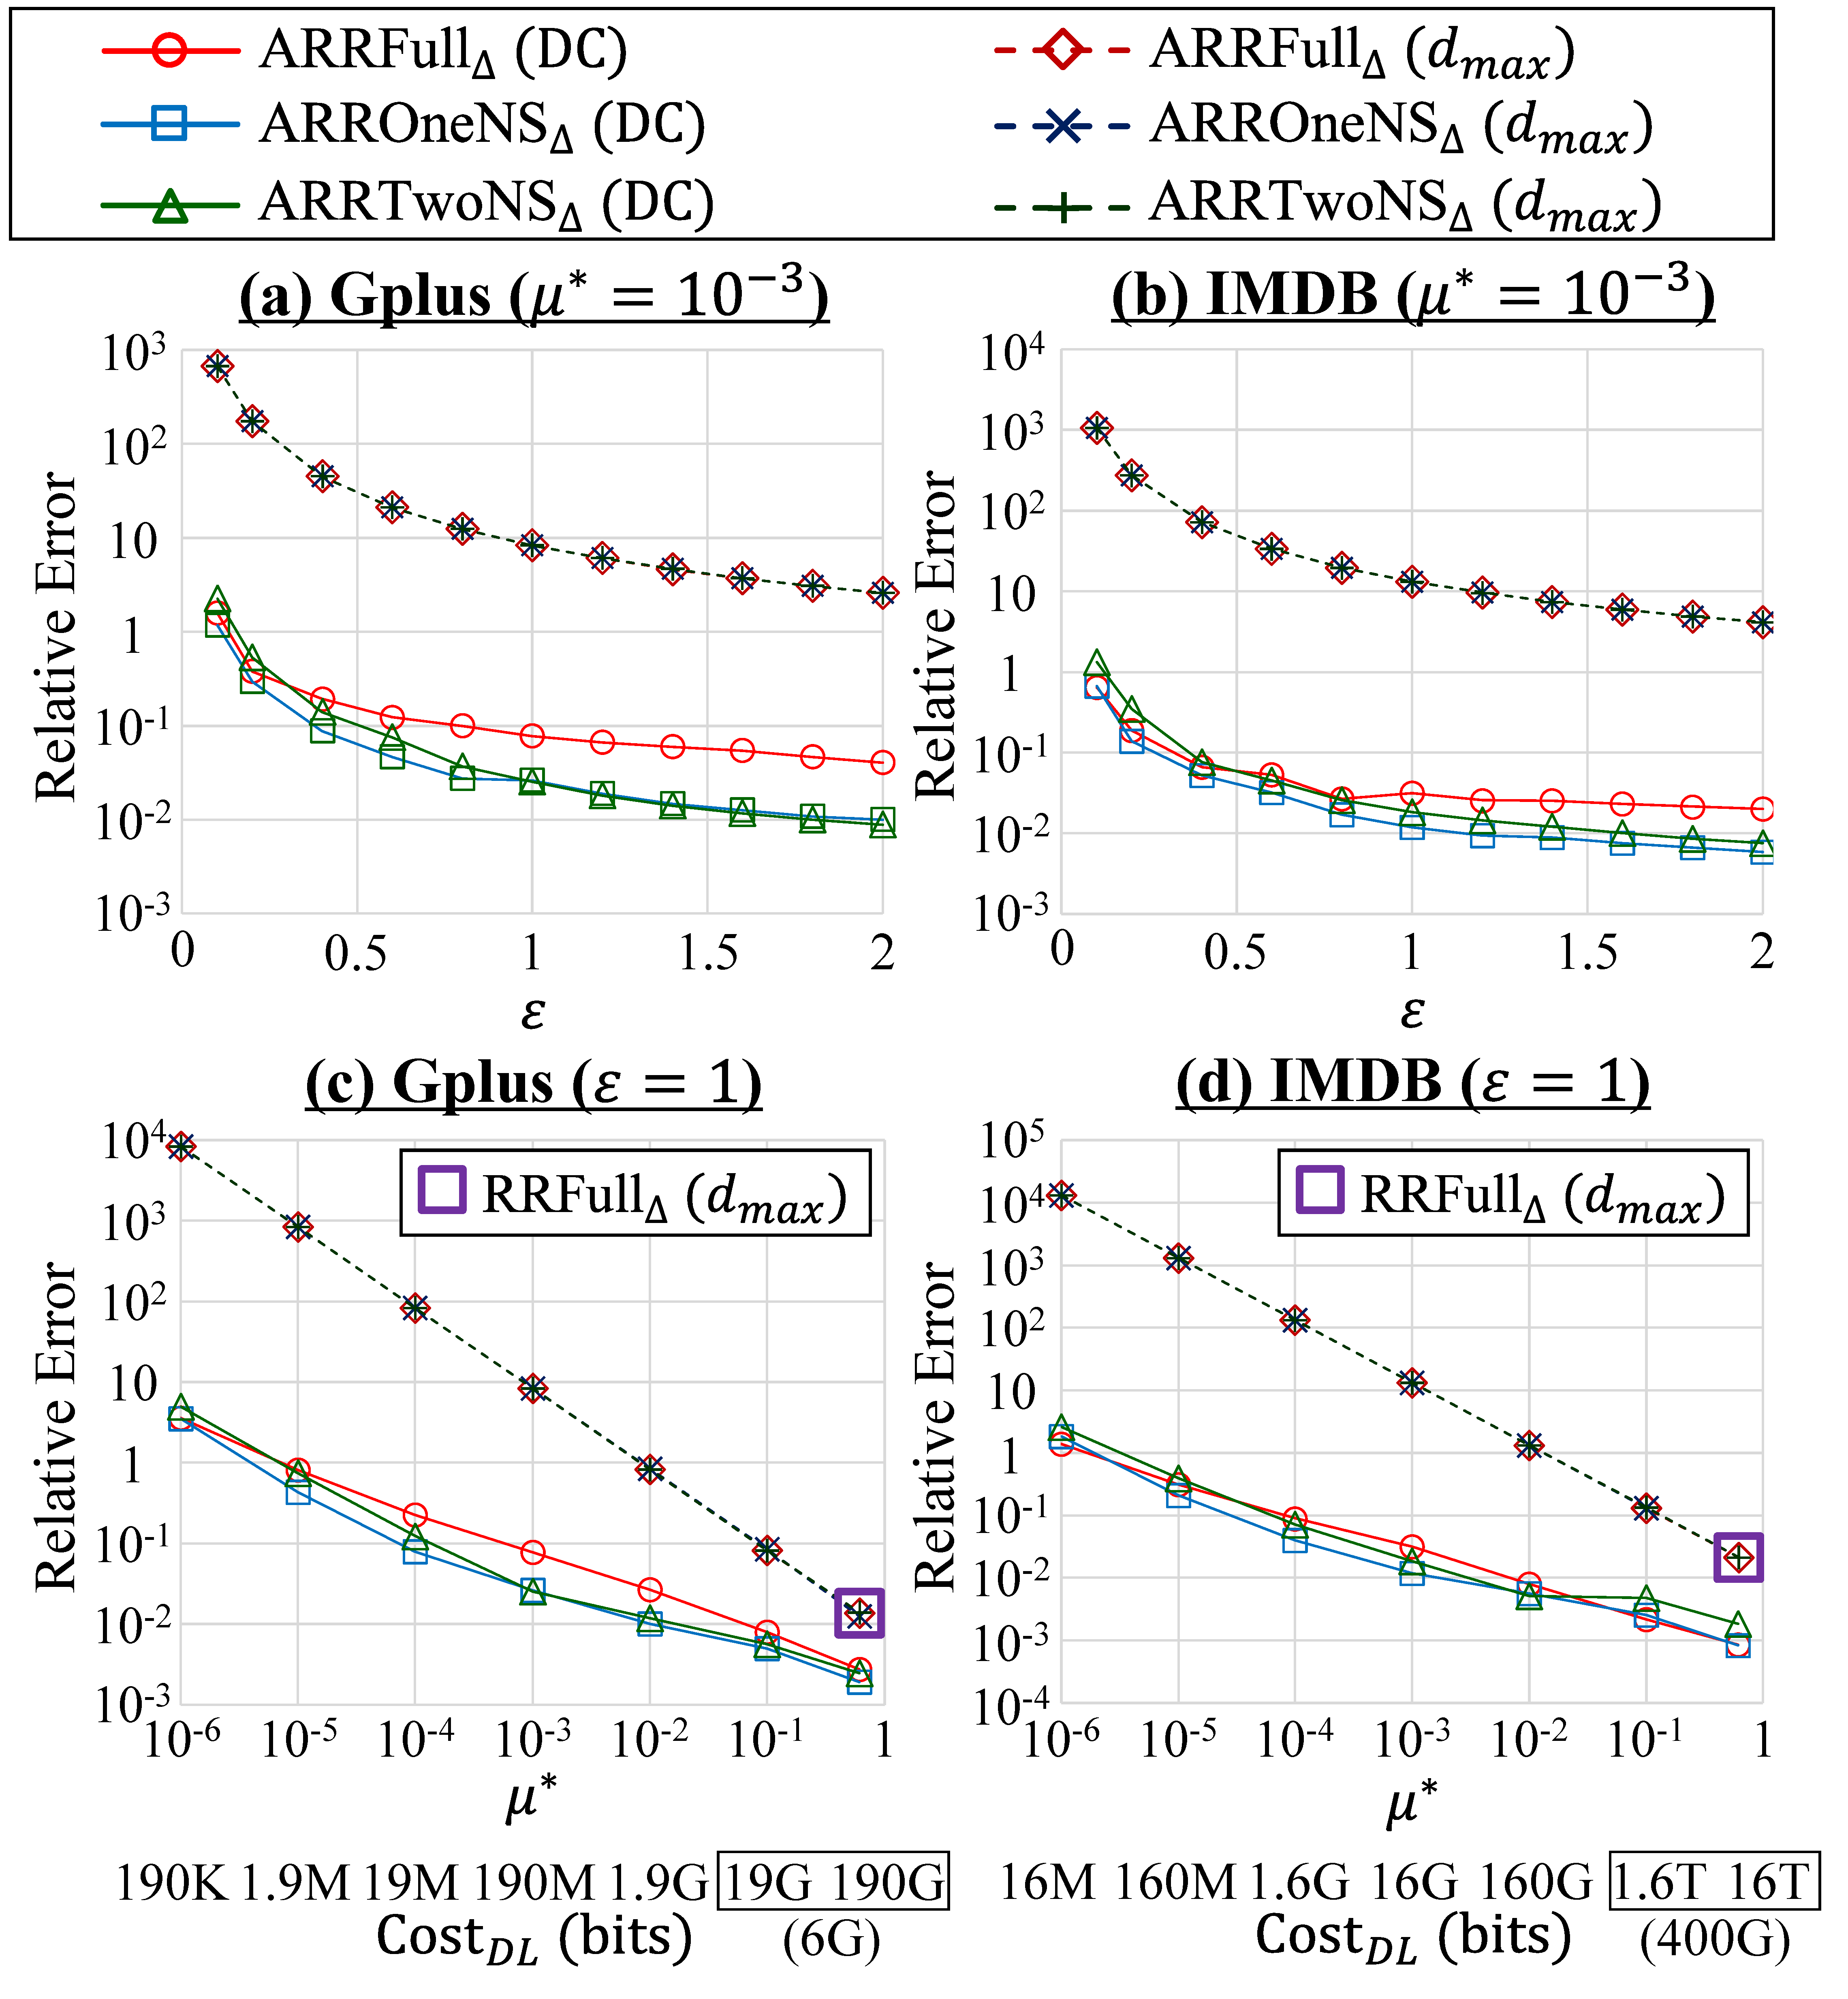
\includegraphics[width=0.99\linewidth]{fig/res2_w_Lap.pdf}
  \vspace{-5mm}
  \caption{Relative error of our three algorithms with (``DC'') or without (``$d_{max}$'') double clipping ($n=107614$ in \GPlus{}, $n=896308$ in \IMDB{}). \AlgSec{} is the 
  %two-rounds 
  algorithm in~\cite{Imola_USENIX21}. 
  $\CostDL$ is 
  %calculated by 
  an upper-bound in 
  (\ref{chap2-eq:CostDL_F}). 
  %Note that 
  When $\mu^* \geq 0.1$, 
  %(marked with squares), 
  $\CostDL$ can be $6$ Gbits and $400$ Gbits in \GPlus{} and \IMDB{}, respectively, by downloading only 0/1 for each pair of users $(v_j,v_k)$.} 
  \label{chap2-fig:res2_w_Lap}
\end{figure}

% \begin{table}[t]
% \caption{Basic notations.} 
% \centering
% \hbox to\hsize{\hfil
% \begin{tabular}{l|l|l}
% \hline
% Algorithm		&	\GPlus{} ($\epsilon=1$) &  \IMDB{}  ($\epsilon=1$)\\
% \hline
% \AlgOne{}   &   $0.078$   &   $0.031$\\
% \hline
% \end{tabular}
% \hfil}
% \label{chap2-tab:res2_w_Lap_abst}
% \end{table}

Figures~\ref{chap2-fig:res2_w_Lap_abst} and \ref{chap2-fig:res2_w_Lap} show the results. 
Figure~\ref{chap2-fig:res2_w_Lap_abst} highlights the relative error of our three algorithms with double clipping when $\epsilon=1$ or $2$ and $\mu^*=10^{-3}$. 
% Figure \ref{chap2-fig:res2_w_Lap} shows the results. 
``DC'' (resp.~``$d_{max}$'') represents algorithms with (resp.~without) double clipping. 
\AlgSec{} (marked with purple square) in Figure~\ref{chap2-fig:res2_w_Lap} (c) and (d) represents the two-rounds algorithm in~\cite{Imola_USENIX21}. 
Note that this is a special case of our \AlgOne{} without sampling ($\mu =\frac{e^{\epsilon_1}}{e^{\epsilon_1}+1} = 0.62$). 
% as described in Section~\ref{chap2-sub:algorithms_overview}. 
Figure~\ref{chap2-fig:res2_w_Lap} (c) and (d) also show the download cost $\CostDL$ calculated by 
(\ref{chap2-eq:CostDL_F}). 
Note that 
when $\mu^* \geq 0.1$ (marked with squares), 
$\CostDL$ can be $6$Gbits and $400$Gbits in \GPlus{} and \IMDB{}, respectively, by downloading only 0/1 for each pair of users $(v_j,v_k)$; $\CostDL = \frac{(n-1)(n-2)}{2}$ in this case. 
% $\CostDL$ is $400$Gbits and $6$Gbits in \GPlus{} and \IMDB{}, respectively, when user $v_i$ downloads only 0/1 for each 
% pair of users $(v_j,v_k)$ ($\CostDL = \frac{(n-1)(n-2)}{2}$ in this case). 

Figures~\ref{chap2-fig:res2_w_Lap_abst} and \ref{chap2-fig:res2_w_Lap} show that our \AlgTwo{} (DC) 
% with double clipping 
provides the best (or almost the best) performance in all cases. 
This is because \AlgTwo{} (DC) introduces the $4$-cycle trick 
% (shown in Figure~\ref{chap2-fig:four-cycle}) 
and effectively reduces the global sensitivity of the Laplacian noise by double clipping. 
% \AlgThree{} (DC) is outperformed by \AlgTwo{} (DC), 
% \AlgTwo{} (DC) outperforms \AlgThree{} (DC), 
% especially when $\epsilon$ or $\mu_F$ ($=\mu_O^2 = \mu_T^3$) is small 
% (e.g., $\epsilon=0.1$ to $0.8$, $\mu_F=10^{-6}$ to $10^{-4}$). 
% There are two reasons for this: 
% (1) \AlgThree{} cannot effectively reduce the global sensitivity by double clipping,
% (2) the Laplacian noise increases with decrease in $\epsilon$ or $\mu_F$, 
% This is because \AlgThree{} cannot effectively reduce the global sensitivity by double clipping and the Laplacian noise increases with decrease in $\epsilon$ or $\mu_F$ 
% and has a non-negligible effect on the estimation error for small $\epsilon$ or $\mu_F$, 
% (as shown in Table~\ref{chap2-tab:privacy_utility_cost} of Section~\ref{chap2-sub:clip_theoretical_analysis}). 
% The difference between \AlgTwo{} (DC) and \AlgOne{} (DC) is also small for very small $\epsilon$ or $\mu_F$ (e.g., $\epsilon=0.1$, $\mu_F=10^{-6}$) because the Laplacian noise is dominant in this case. 
% Later, we will also 
% provide a detailed investigation of the relation between the Laplacian noise and the relative error while changing $n$. 
% to answer our research question RQ1. 
Later, we will 
% also 
% provide a detailed investigation of 
investigate 
the effectiveness of the $4$-cycle trick in detail 
by not adding the Laplacian noise. 
% and 
We will also investigate 
%the relation between the Laplacian noise and the relative error 
the impact of the Laplacian noise 
while changing $n$. 

Figure~\ref{chap2-fig:res2_w_Lap} also shows that 
the relative error is almost the same between our three algorithms without double clipping (``$d_{max}$'') and that it is too large. 
% the relative error of our three algorithms without double clipping is too large and that it is almost the same between the three. 
This is because $\Lap(\frac{d_{max}}{\epsilon_2}$) is too large and dominant. 
The relative error is significantly reduced by introducing our double clipping in all cases. 
% For example, our \AlgTwo{} (DC) without sampling ($\mu_F =\frac{e^{\epsilon_1}}{e^{\epsilon_1}+1}$)
For example, when $\mu^* = 10^{-3}$, our double clipping reduces the relative error of \AlgTwo{} by two or three orders of magnitude. 
% \AlgTwo{} (DC) also reduces the expected download size by $\mu_F = \mu_O^2 = 10^{-3}$ while keeping roughly the same relative error as the algorithm in~\cite{Imola_USENIX21}, thanks to double clipping. 
The improvement is larger for smaller $\mu^*$. 

In \conference{the full version \cite{Imola_arXiv22}}\arxiv{Appendix~\ref{chap2-sec:EC_DC}}, we also evaluate the effect of edge clipping and noisy triangle clipping independently and show that each component significantly reduces the relative error. 

\smallskip
\noindent{\textbf{Communication Cost.}}~~From Figure~\ref{chap2-fig:res2_w_Lap} (c) and (d), we can explain how much our algorithms can reduce the download cost while keeping high utility, e.g., relative error $\ll 1$. 

For example, when we use the algorithm in \cite{Imola_USENIX21}, the download cost is 
$\CostDL = 400$ Gbits in \IMDB{}. 
% $\CostDL = 400$ Gbits and $6$ Gbits in \GPlus{} and \IMDB{}, respectively. 
Thus, when the download speed is $20$ Mbps 
% (which is a 
(recommended speed in YouTube \cite{YouTube_speed}), every user $v_i$ needs 6 hours to download the message $M_i$, which is far from practical. 
In contrast, our \AlgTwo{} (DC) can reduce it to 
% $100$ 
$160$ 
Mbits (8 seconds when $20$ Mbps download rate) or less 
while keeping relative error $= 0.21$, 
% (relative error $= 0.21$), 
% or $1$ Gbits (relative error $= 0.040$). 
% Consequently, every user needs only 
% 5 
% 8 
% or 50 
% seconds or less, 
which is practical and a dramatic improvement over \cite{Imola_USENIX21}. 
% Therefore, private triangle counting is now practical.

We also note that since $d_{max} \ll n$ in \IMDB{}, 
% the ARR outputs ``1'' with probability $\mu e^{-\epsilon_1}$ in most cases
% the download cost 
$\CostDL$ of our \AlgTwo{} (DC) 
can also be roughly approximated by $60$ Mbits (3 seconds) by replacing $\mu$ with $\mu e^{-\epsilon_1}$ in 
(\ref{chap2-eq:CostDL_F}). 
%(\ref{chap2-eq:CostDL_O}). 

% We also note that the upload cost is much smaller; e.g., by (\ref{chap2-eq:CostUL_proposal}), $\CostUL{} = 11$ Mbits in \IMDB{} even when $\mu=1$. 
% Thus, it is not an issue.

\smallskip
% \noindent{\textbf{Three Algorithms w/o Lap.}}~~
\noindent{\textbf{4-Cycle Trick.}}~~We 
% first evaluated 
also investigated 
% how well our two algorithms \AlgTwo{} and \AlgThree{} address the $4$-cycle issue of \AlgOne{} 
the effectiveness of our $4$-cycle trick in \AlgTwo{} and \AlgThree{} 
% (shown in Figure~\ref{chap2-fig:four-cycle}) 
in detail. 
% explained in Section~\ref{chap2-sub:algorithms_overview}. 
% the relation between the $4$-cycle issue 
To this end, we evaluated our three algorithms when we did \textit{not} add the Laplacian noise at the second round. 
% (i.e., $\epsilon_2 = \infty$). 
Note that they do not provide edge LDP, as $\epsilon_2 = \infty$. 
The purpose here is to purely investigate the effectiveness of the $4$-cycle trick 
% issue 
related to our first research question RQ1. 
% We will report experimental results of the three algorithms with the Laplacian noise later. 

\begin{figure}[t]
  \centering
  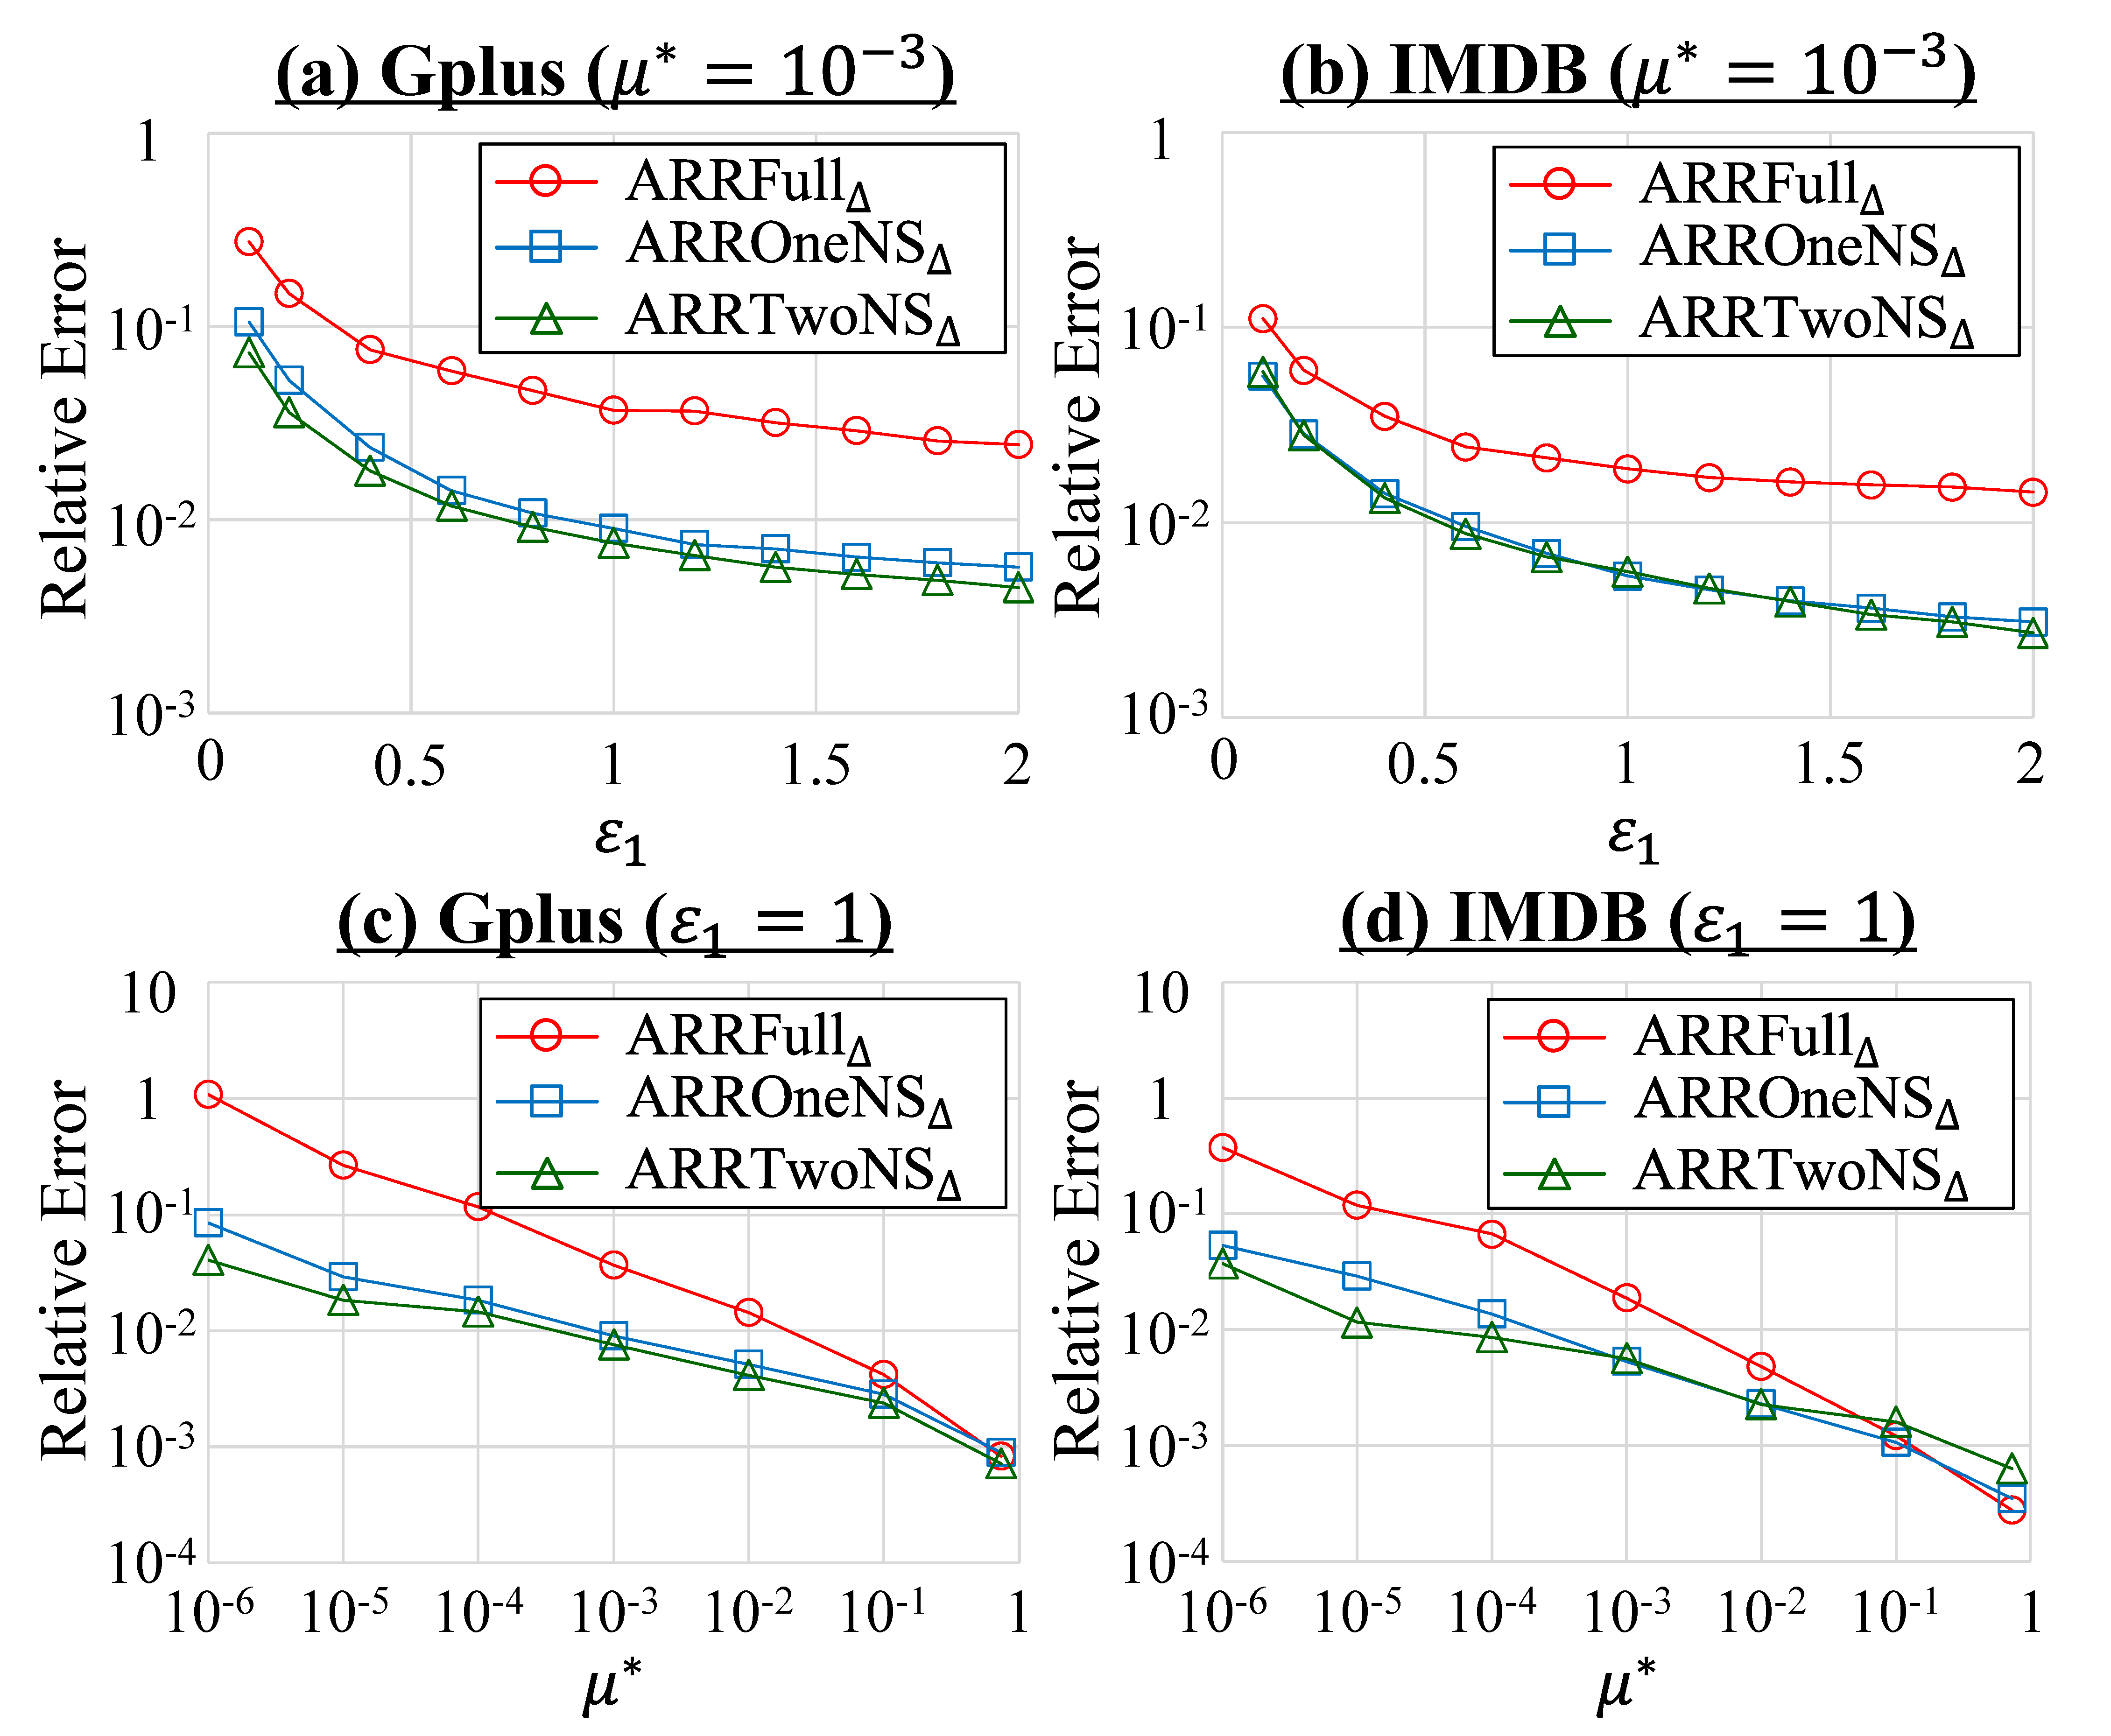
\includegraphics[width=0.99\linewidth]{fig/res1_wo_Lap.pdf}
  \vspace{-5mm}
  \caption{Relative error of our three algorithms without the Laplacian noise 
  % at the second round 
  ($n=107614$ in \GPlus{}, $n=896308$ in \IMDB{}).} 
  \label{chap2-fig:res1_wo_Lap}
\end{figure}

% We first evaluated our three triangle counting algorithms with double clipping. 
Figure~\ref{chap2-fig:res1_wo_Lap} shows the results, where 
% $\mu_F$ (resp.~$\epsilon_1$) is changed from $10^{-6}$ to $1$ (resp.~$0.1$ to $2$). 
% $\epsilon_1$ (resp.~$\mu_F$) is changed from $0.1$ to $2$ (resp.~$10^{-6}$ to $\frac{e^{\mu_F}}{e^{\mu_F} + 1}$). 
$\epsilon_1$ and 
% $\mu_F$ ($= \mu_O^2 = \mu_T^3$) 
$\mu^*$ 
are changed to various values. 
Figure~\ref{chap2-fig:res1_wo_Lap} shows that \AlgTwo{} and \AlgThree{} significantly outperform \AlgOne{} when 
% $\mu_F$ 
$\mu^*$ 
is small. 
This is because in both \AlgTwo{} and \AlgThree{}, 
% the first term in the expected $l_2$ loss 
the factors of 
% $S_3$ (\#3-stars) and $P_3$ (\#3-paths) 
$C_4$ (\#4-cycles) and $S_3$ (\#3-stars) 
in the expected $l_2$ loss 
diminish 
for small $\mu$, 
% as 
% $\mu_F$ ($= \mu_O^2 = \mu_T^3$) 
% the parameter $\mu$ in the ARR 
% goes to $0$, 
as explained in Section~\ref{chap2-sub:algorithms_theoretical_analysis}. 
In other words, \AlgTwo{} and \AlgThree{} effectively address the $4$-cycle issue. 
Figure~\ref{chap2-fig:res1_wo_Lap} also shows that \AlgThree{} slightly outperforms \AlgTwo{} when $\mu^*$ is small. 
% (e.g., $10^{-6}$ to $10^{-4}$). 
This is because 
% the first term in the expected $l_2$ loss diminishes 
% the factors of $S_3$ and $P_3$ 
the factors of $C_4$ and $S_3$ 
diminish 
more rapidly; i.e., \AlgThree{} addresses the $4$-cycle issue more aggressively. 

However, when we add the Laplacian noise, \AlgThree{} (DC) is outperformed by \AlgTwo{} (DC), as shown in Figure~\ref{chap2-fig:res2_w_Lap}. 
% \AlgTwo{} (DC) outperforms \AlgThree{} (DC), 
% especially when $\epsilon$ or $\mu_F$ ($=\mu_O^2 = \mu_T^3$) is small 
% (e.g., $\epsilon=0.1$ to $0.8$, $\mu_F=10^{-6}$ to $10^{-4}$). 
This is because \AlgThree{} cannot effectively reduce the global sensitivity by double clipping. 
In Figure~\ref{chap2-fig:res2_w_Lap}, the difference between \AlgTwo{} (DC) and \AlgOne{} (DC) is also small for very small $\epsilon$ or $\mu^*$ (e.g., $\epsilon=0.1$, $\mu^*=10^{-6}$) because the Laplacian noise is dominant in this case. 
% (as shown in Table~\ref{chap2-tab:privacy_utility_cost} of Section~\ref{chap2-sub:clip_theoretical_analysis}). 

\smallskip
\noindent{\textbf{Changing $\bm{n}$.}}~~We 
finally 
% also 
evaluated our three algorithms with double clipping while changing the number $n$ of users. 
In both \GPlus{} and \IMDB{}, we randomly selected $n$ users from all users and extracted a graph with $n$ users. 
Then we evaluated the relative error while changing $n$ to various values.

\begin{figure}[t]
  \centering
  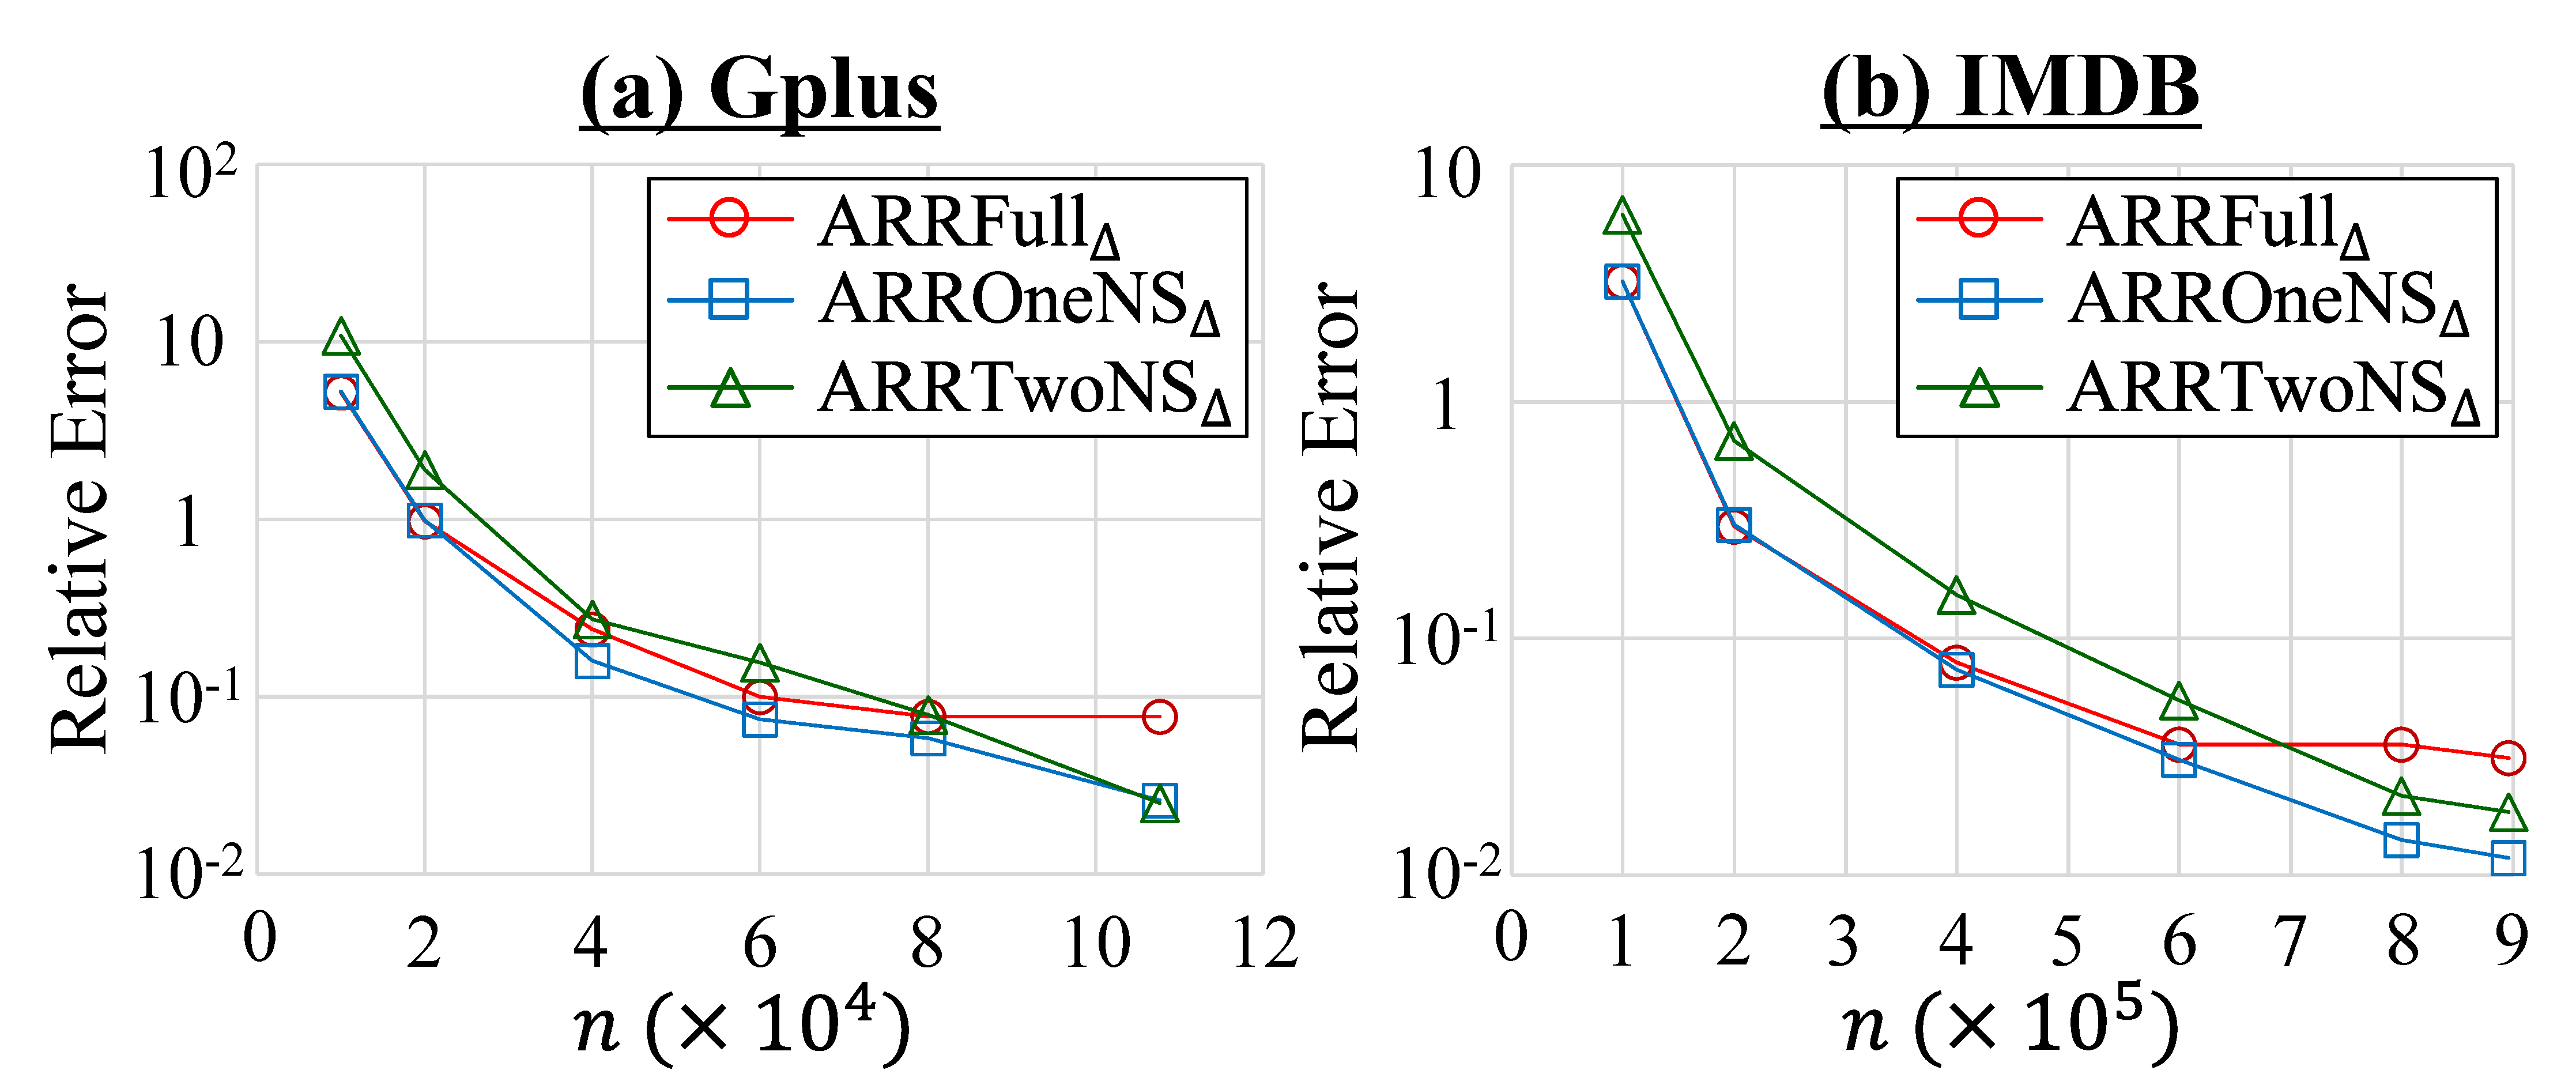
\includegraphics[width=0.99\linewidth]{fig/res3_n.pdf}
  \vspace{-4mm}
  \caption{Relative error of our three algorithms with double clipping for various values of $n$ 
  ($\epsilon=1$, $\mu^*=10^{-3}$).} 
  \label{chap2-fig:res3_n}
\end{figure}

Figure~\ref{chap2-fig:res3_n} shows the results, where $\epsilon=1$ ($\epsilon_0=0.1$, $\epsilon_1 = \epsilon_2 = 0.45$) and $\mu^* = 10^{-3}$. 
In all 
% the 
three algorithms, the relative error decreases with increase in $n$.
This is because the expected $l_2$ loss can be expressed as 
% $O(n)$ (when we regard $\epsilon$ and $\mu_F$ as constants and ignore $d_{max}$) 
$O(n d_{max}^3)$ or $O(n d_{max}^2)$ 
% (when we regard $\epsilon$ as constants) 
in these algorithms as shown in Section~\ref{chap2-sub:clip_theoretical_analysis} and the square of the true triangle count can be expressed as $\Omega(n^2)$.
In other words, when $d_{max} \ll n$, the relative error becomes smaller for larger $n$. 
% In other words, this is consistent with our theoretical results. 
Figure~\ref{chap2-fig:res3_n} also shows that for small $n$, \AlgThree{} provides the worst performance and 
\AlgTwo{} performs almost the same as \AlgOne{}. 
% the difference between \AlgTwo{} and \AlgOne{} is very small. 
For large $n$, 
% \AlgThree{} outperforms \AlgOne{} and 
\AlgOne{} performs the worst and 
\AlgTwo{} performs the best. 


To investigate the reason for this, we decomposed the estimation error into two components -- 
the first error caused by empirical estimation and the second error caused by the Laplacian noise. 
Specifically, for each algorithm, 
we evaluated the first error by calculating the relative error when we did not add the Laplacian noise ($\epsilon_1 = 0.45$). 
Then we evaluated the second error by subtracting the first error from the relative error when we used double clipping ($\epsilon_0=0.1$, $\epsilon_1 = \epsilon_2 = 0.45$). 

Figure~\ref{chap2-fig:res3_emp_Lap} shows the results for some values of $n$, where ``emp'' represents the first error by empirical estimation and ``Lap'' represents the second error by the Laplacian noise. 
We observe that the second error 
rapidly decreases with increase in $n$. 
% The difference between \AlgOne{} and \AlgTwo{} 
% This is because the expected $l_2$ loss of the Laplacian noise is $O(\sum_{i=1}^n \kappa_i^2)$, 
% which is much smaller than $O(n d_{max}^2)$, 
% as shown in Section~\ref{chap2-sub:clip_theoretical_analysis}. 
In addition, 
% Figure~\ref{chap2-fig:res3_emp_Lap} also shows that 
the first error of \AlgOne{} is much larger than those of \AlgTwo{} and \AlgThree{} when $n$ is large. 

We also examined 
% the maximum degree $d_{max}$ and 
the number $C_4$ of $4$-cycles as a function of $n$. Figure~\ref{chap2-fig:res4_4cycles} shows the results. 
We observe that $C_4$ (which is $O(n d_{max}^3)$) is quartic in $n$; e.g., $C_4$ is increased by $2^4 \approx 10$ and $6^4 \approx 10^3$ when $n$ is multiplied by $2$ and $6$, respectively. 
This is because we randomly selected $n$ users from all users and $d_{max}$ is almost proportional to $n$ (though $d_{max} \ll n$). 
% We observe that $d_{max}$ is proportional to $n$ (though $d_{max} \ll n$). 
% This is because we randomly selected $n$ users from all users. 
% Consequently, $C_4$ which can be expressed as $O(n d_{max}^3)$ is quartic in $n$; e.g., $C_4$ is increased by $2^4 \approx 10$ and $6^4 \approx 10^3$ when $n$ is multiplied by $2$ and $6$, respectively. 

\begin{figure}[t]
  \centering
  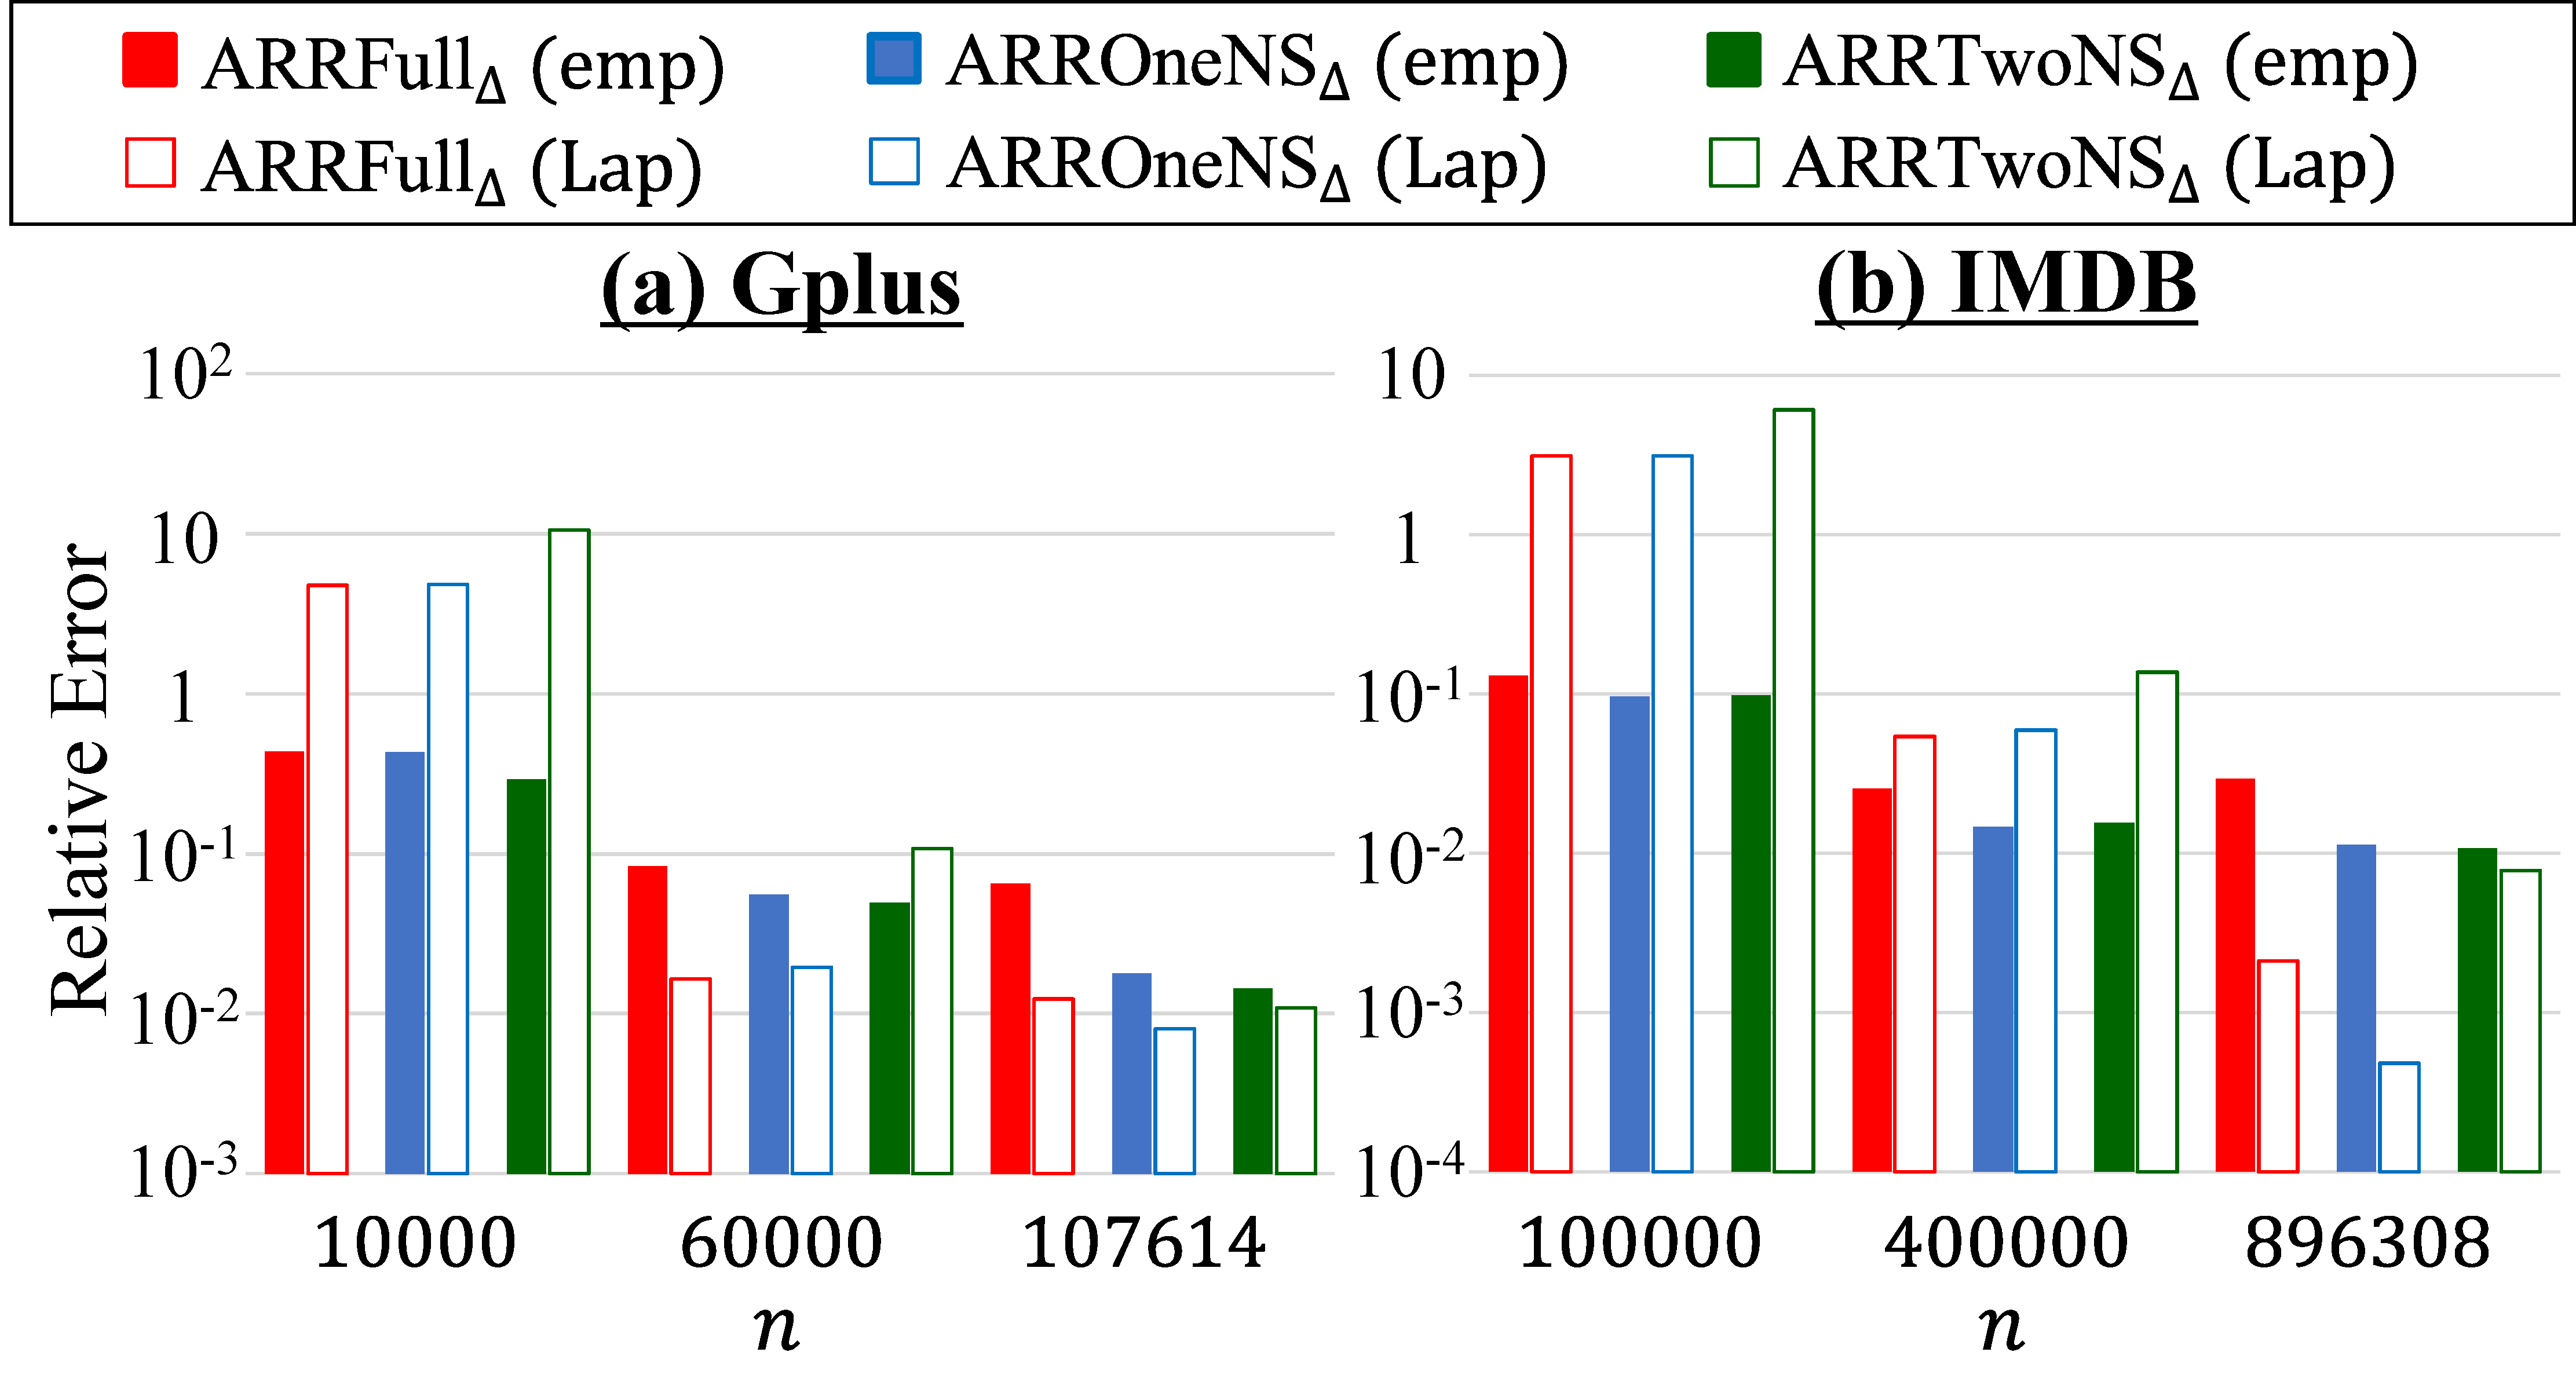
\includegraphics[width=0.99\linewidth]{fig/res3_emp_Lap.pdf}
  \vspace{-5mm}
  \caption{Relative error of empirical estimation and the Laplacian noise in our three algorithms with double clipping ($\epsilon=1$, $\mu^*=10^{-3}$).} 
  \label{chap2-fig:res3_emp_Lap}
% \end{figure}
 \vspace{1mm}
% \begin{figure}[t]
  \centering
  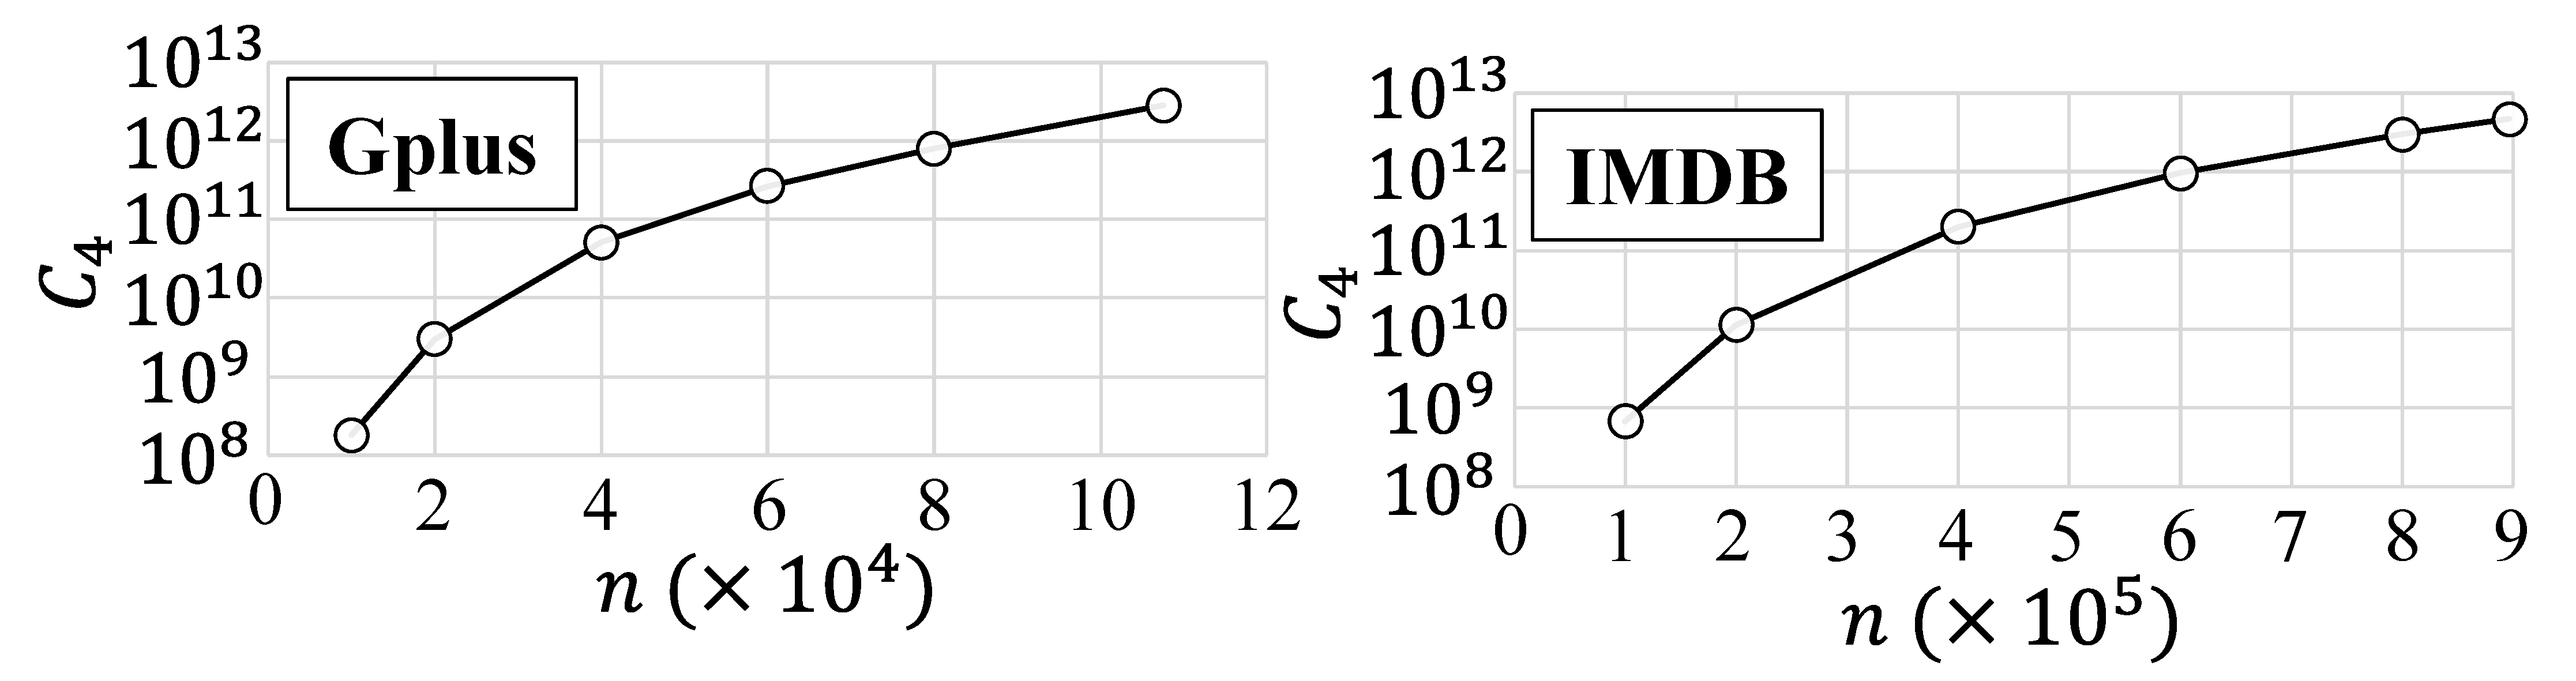
\includegraphics[width=0.99\linewidth]{fig/res4_4cycles.pdf}
  \vspace{-5mm}
%   \caption{Maximum degree $d_{max}$ and \#$4$-cycles $C_4$.} 
  \caption{\#$4$-cycles $C_4$.} 
  \label{chap2-fig:res4_4cycles}
\end{figure}

Based on Figures~\ref{chap2-fig:res3_emp_Lap} and \ref{chap2-fig:res4_4cycles}, we can explain 
% the results in 
Figure~\ref{chap2-fig:res3_n} as follows. 
As shown in Section~\ref{chap2-sub:clip_theoretical_analysis}, the $l_2$ loss of empirical estimation can be expressed as 
% $O(\frac{n d_{max}^3}{\mu_F})$, $O(\frac{n d_{max}^2}{\mu_O^2})$, and $O(\frac{n d_{max}^2}{\mu_T^3})$ 
$O(n d_{max}^3)$, $O(n d_{max}^2)$, and $O(n d_{max}^2)$ 
in \AlgOne{}, \AlgTwo{}, and \AlgThree{}, respectively. 
% when 
% we regard $\epsilon$ as a constant.
% $\mu_F$ ($= \mu_O^2 = \mu_T^3$) 
% $\mu^*$ is small.  
The large $l_2$ loss of \AlgOne{} is caused by a large value of $C_4$. 
% as shown in Figure~\ref{chap2-fig:res4_4cycles}. 
% the $4$-cycle issue. 
% When 
% $\mu_F$ is small, 
% $n$ is small, 
% the Laplacian noise has a non-negligible impact on the estimation error. 
% as explained in Section~\ref{chap2-sub:clip_theoretical_analysis}. 
% However, 
The expected $l_2$ loss of the Laplacian noise is 
$O(\sum_{i=1}^n \kappa_i^2)$, 
% $O(\sum_{i=1}^n \lambda_i^2 \td_i^2)$, 
which is much smaller than $O(n d_{max}^2)$. 
Thus, 
% when $n$ is large, 
as $n$ increases, 
% when $d_{max}$ is proportional to $n$, 
% as in Figure~\ref{chap2-fig:res4_4cycles}, 
the Laplacian noise becomes relatively very small, 
% rapidly decreases with increase in $n$ 
as shown in Figure~\ref{chap2-fig:res3_emp_Lap}. 
Consequently, \AlgTwo{} provides the best performance for large $n$ because it addresses the $4$-cycle issue 
and effectively reduces the global sensitivity. 
This explains the results in Figure~\ref{chap2-fig:res3_n}. 
It is also interesting that when $n \approx 10^5$, \AlgOne{} performs the worst in \GPlus{} and almost the same as \AlgTwo{} in \IMDB{} (see Figure~\ref{chap2-fig:res3_n}). 
This is because \GPlus{} is more dense than \IMDB{} 
% (as described in Section~\ref{chap2-sub:setup}) 
and $C_4$ is much larger in \GPlus{} when $n \approx 10^5$, as in Figure~\ref{chap2-fig:res4_4cycles}.

In other words, Figures~\ref{chap2-fig:res3_n}, \ref{chap2-fig:res3_emp_Lap}, and \ref{chap2-fig:res4_4cycles} are consistent with our theoretical results in Section~\ref{chap2-sub:clip_theoretical_analysis}. 
From these results, we conclude that \AlgTwo{} is effective especially for 
a large graph (e.g., $n \approx 10^6$) or dense graph (e.g., \GPlus{}) where the number $C_4$ of $4$-cycles is large. 
% a graph that has a large number of $4$-cycles. 
% In Appendix~\ref{chap2-sec:BAmodel}, we also show similar results using the Barab\'{a}si-Albert graph model.



% \smallskip
% \noindent{\textbf{Communication Cost.}}~~TBD.

\smallskip
\noindent{\textbf{Summary.}}~~In summary, our answers to our three research questions RQ1-3 
% at the beginning of Section~\ref{chap2-sec:experiments} 
are as follows. 
% \begin{itemize}
%     \item Our 
% \end{itemize}
% First, 
[RQ1]: Our \AlgTwo{} achieves almost the smallest estimation error in all cases and outperforms the other two, especially for a large graph or dense graph where $C_4$ is large. 
[RQ2]: Our double clipping reduces the estimation error by two or three orders of magnitude. 
[RQ3]: Our entire algorithm (\AlgTwo{} with double clipping) dramatically reduces the communication cost, 
e.g., 
% from $400$ Gbits to $160$ Mbits or less (relative error $=0.21$) in \IMDB{}.
% When the DL speed is $20$ Mbps \cite{YouTube_speed}, the DL time is reduced from $6$ hours to $5$ seconds. 
from $6$ hours to $8$ seconds or less (relative error $=0.21$) in \IMDB{} at a $20$ Mbps download rate \cite{YouTube_speed}. 

Thus, triangle counting under edge LDP is now 
much more 
practical. 
In Appendix~\ref{chap2-sec:cluster}, we show that the clustering coefficient can also be accurately estimated using our algorithms.
